\section{Result 3: the learning curve of logistic regression}
\label{sec:result-3}

Unregularized logistic regression: $\hat\theta_n=\argmin_\theta\hat L_n(\theta)$,
$\hat L_n(\theta)=\frac1n\sum_i\ell(\theta;x_i,y_i)$, $\ell(\theta;x,y)=\ln(1+e^{-y\,\theta\cdot x})$,
$\theta\in\R^p$ ($p=k+1$), $\phi$ the sigmoid, $L(\theta)=\E_Q\ell(\theta;x,y)$ and
$\theta^\star=\argmin L$. Unlike Results~1 and 2 this is not a bound but a prediction of the
learning curve itself.

\begin{theorem}[Result 3]
\label{thm:3}
Let $H=\E[\phi(\theta^\star\cdot x)\phi(-\theta^\star\cdot x)\,xx^\top]$ and $G=\E[\nabla\ell\,\nabla\ell^\top]$
at $\theta^\star$, with $\nabla\ell=-\phi(-y\,\theta^\star\cdot x)\,y\,x$. If $\theta^\star$ exists,
$\hat\theta_n\to\theta^\star$ in probability and $H\succ0$, then
\[ \sqrt n(\hat\theta_n-\theta^\star)\xrightarrow{d}N(0,H^{-1}GH^{-1}),\qquad
   n\bigl(L(\hat\theta_n)-L(\theta^\star)\bigr)\xrightarrow{d}\tfrac12Z^\top HZ,\quad Z\sim N(0,H^{-1}GH^{-1}), \]
and the limit has mean $\Tr(H^{-1}G)/2$, which gives the prediction
$\E[L(\hat\theta_n)-L(\theta^\star)]\approx\Tr(H^{-1}G)/(2n)$. If the model is well specified,
$G=H$ and the prediction is $p/(2n)$, so $\Tr(H^{-1}G)/p$ measures misspecification.
\end{theorem}

\begin{proof}
\emph{Derivatives.} With $t=\theta\cdot x$, $\frac{d}{dt}\ln(1+e^{-yt})=-y\,\phi(-yt)$, so
$\nabla\ell=-\phi(-y\,\theta\cdot x)\,y\,x$; differentiating again and using $y^2=1$ and
$\phi(-yt)\phi(yt)=\phi(t)\phi(-t)$, $\nabla^2\ell=g(\theta\cdot x)\,xx^\top$ with $g(t)=\phi(t)\phi(-t)$.
Its expectation at $\theta^\star$ is $H$.

\emph{Assumptions.} $\theta^\star$ exists because the population is not linearly separable (the
classes overlap); training samples that \emph{are} separable have no minimizer and are excluded.
Consistency of $\hat\theta_n$ is the standard consistency of M-estimators \citep{vandervaart1998asymptotic}; here
$\hat L_n$ is convex and $\theta^\star$ is unique because $\nabla^2L\succ0$ everywhere.
$H\succ0$ because the features are not supported on a hyperplane and $g>0$. $G$ is finite because
$\norm{\nabla\ell}\le\norm x\le1$. The Hessian is Lipschitz: $g'=g(1-2\phi)$ and $\abs{g'}\le1/(6\sqrt3)\le1$,
so $\norm{\nabla^2\ell(\theta)-\nabla^2\ell(\theta')}\le\abs{(\theta-\theta')\cdot x}\norm x^2\le\norm{\theta-\theta'}$.

\emph{Asymptotic normality.} Since $\nabla\hat L_n(\hat\theta_n)=0$, Taylor's theorem in integral
form gives $0=\nabla\hat L_n(\theta^\star)+\bar H_n(\hat\theta_n-\theta^\star)$ with
$\bar H_n=\int_0^1\nabla^2\hat L_n(\theta^\star+s(\hat\theta_n-\theta^\star))\,ds$. By the Lipschitz
bound, $\norm{\bar H_n-\nabla^2\hat L_n(\theta^\star)}\le\norm{\hat\theta_n-\theta^\star}\to0$, and
$\nabla^2\hat L_n(\theta^\star)\to H$ by the law of large numbers, so $\bar H_n\to H$ in probability
and is invertible with probability tending to 1. The summands of $\nabla\hat L_n(\theta^\star)$
are i.i.d.\ with mean $\nabla L(\theta^\star)=0$ and covariance $G$, so by the central limit
theorem $\sqrt n\,\nabla\hat L_n(\theta^\star)\to N(0,G)$, and by Slutsky's lemma
$\sqrt n(\hat\theta_n-\theta^\star)=-\bar H_n^{-1}\sqrt n\,\nabla\hat L_n(\theta^\star)\to N(0,H^{-1}GH^{-1})$:
the sandwich covariance.

\emph{Excess risk.} $\nabla L(\theta^\star)=0$ and $\nabla^2L$ is Lipschitz with constant 1, so
with $v=\hat\theta_n-\theta^\star$,
\[ \abs{L(\hat\theta_n)-L(\theta^\star)-\tfrac12v^\top Hv}\le\tfrac16\norm v^3. \]
Multiplying by $n$, the remainder is $O_P(n^{-1/2})$ and $n\cdot\frac12v^\top Hv\to\frac12Z^\top HZ$ by
the continuous mapping theorem. Its mean is $\frac12\Tr(H\,H^{-1}GH^{-1})=\frac12\Tr(H^{-1}G)$.
Reading this limit mean as the mean of $n(L(\hat\theta_n)-L(\theta^\star))$ at finite $n$ is the
approximation that the experiment tests.

\emph{Well specified.} If $P(y=1\mid x)=\phi(\theta^\star\cdot x)$, then with $t=\theta^\star\cdot x$,
$\E[\phi(-yt)^2\mid x]=\phi(t)\phi(-t)^2+\phi(-t)\phi(t)^2=\phi(t)\phi(-t)$, so $G=H$ and
$\Tr(H^{-1}G)=p$.
\end{proof}

\begin{inshort}
\begin{enumerate}[leftmargin=*]
  \item Gradient $-\phi(-y\theta\cdot x)yx$, Hessian $\phi\phi\,xx^\top$, Lipschitz because $\norm x\le1$.
  \item One Newton step from $\theta^\star$: $\hat\theta-\theta^\star\approx-H^{-1}\nabla\hat L(\theta^\star)$;
    CLT on the gradient (mean 0, covariance $G/n$) gives the sandwich $H^{-1}GH^{-1}/n$.
  \item The excess risk is half the squared $H$-norm: $\frac12\E\,v^\top Hv=\Tr(H^{-1}G)/2n$.
  \item Well specified $\Rightarrow G=H\Rightarrow p/2n$.
\end{enumerate}
\end{inshort}

\paragraph{Measured vs.\ theory (E3).} Overlapping regime; PCA-$k$ CNN features, $k\in\{4,16,64\}$;
$\EThreeRepeats$ repeats on fresh dies, $n\in\{10,20,50,100,300\}\times p$. $\theta^\star$ is fitted on
$\EThreeNPop$ population candidates (which biases the measured excess low by at most
$\EThreePopBias$), $H$ and $G$ on the disjoint test pool. The measured quantity is
$n(L_{\text{test}}(\hat\theta_n)-L_{\text{test}}(\theta^\star))$. The check fixed before running,
measured/predicted in $[0.9,1.1]$ at the largest $n$, holds for all three feature sets.

\begin{center}
\small
\begin{tabular}{lccccccc}
\toprule
& & \multicolumn{2}{c}{prediction for $n\cdot$excess} & \multicolumn{2}{c}{measured at $n=300p$} & & \\
\cmidrule(lr){3-4}\cmidrule(lr){5-6}
features & $p$ & $\Tr(H^{-1}G)/2$ & $p/2$ & mean $\pm$ se & ratio & in $\pm10\%$ from & Wald cov. \\
\midrule
PCA-4 & $\EThreePcaFourP$ & $\EThreePcaFourPred$ & $\EThreePcaFourPHalf$ & $\EThreePcaFourMeasLast\pm\EThreePcaFourSeLast$ & $\EThreePcaFourRatioLast$ & $\EThreePcaFourFromNP\,p$ & $\EThreePcaFourCoverage$ \\
PCA-16 & $\EThreePcaSixteenP$ & $\EThreePcaSixteenPred$ & $\EThreePcaSixteenPHalf$ & $\EThreePcaSixteenMeasLast\pm\EThreePcaSixteenSeLast$ & $\EThreePcaSixteenRatioLast$ & $\EThreePcaSixteenFromNP\,p$ & $\EThreePcaSixteenCoverage$ \\
PCA-64 & $\EThreePcaSixtyFourP$ & $\EThreePcaSixtyFourPred$ & $\EThreePcaSixtyFourPHalf$ & $\EThreePcaSixtyFourMeasLast\pm\EThreePcaSixtyFourSeLast$ & $\EThreePcaSixtyFourRatioLast$ & $\EThreePcaSixtyFourFromNP\,p$ & $\EThreePcaSixtyFourCoverage$ \\
\bottomrule
\end{tabular}
\end{center}

At $n=10p$ the measured excess is $\EThreePcaSixteenRatioFirst$--$\EThreePcaFourRatioFirst$ times the
prediction, and the ratio enters the $\pm10\%$ band from $n=\EThreePcaFourFromNP\,p$ to
$\EThreePcaSixteenFromNP\,p$. At $n=300p$ the sandwich covariance holds as well ($n$ times the
covariance of $\hat\theta_n$ over the repeats has $\EThreePcaFourCovTraceLast$--$\EThreePcaSixtyFourCovTraceLast$
times the trace of $H^{-1}GH^{-1}$), and Wald intervals from each run's own sandwich estimate reach
nominal coverage (at $n=10p$ they under-cover, down to $\EThreePcaSixtyFourCoverageFirst$). The
model is mildly misspecified ($\Tr(H^{-1}G)/p=\EThreePcaFourMiss$--$\EThreePcaSixteenMiss$), so the
shortcut $p/2n$ would be off by under 10\%.

\begin{figure}[tb]
  \centering
  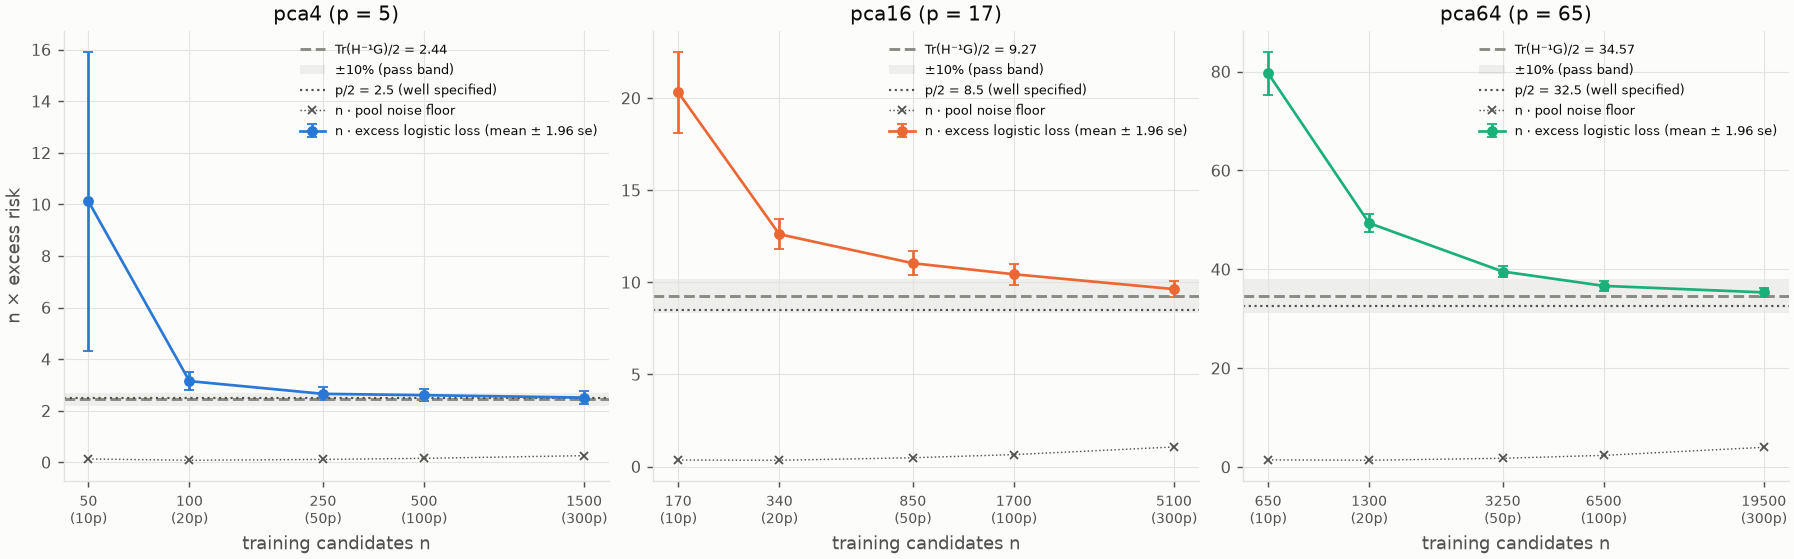
\includegraphics[width=0.8\linewidth]{../figures/e3_learning_curve.png}
  \caption{E3: $n\cdot$excess logistic loss (mean $\pm1.96$ se) with the prediction
  $\Tr(H^{-1}G)/2$ (dashed), its $\pm10\%$ band, $p/2$ (dotted) and $n$ times the pool noise floor.}
  \label{fig:e3}
\end{figure}

\subsection{Result 3b: what more labels will buy}
\label{sec:result-3b}

Result~3 needs $H$ and $G$ at $\theta^\star$, which are population quantities. With $n$ labels in
hand, the practical question is how much $m$ times as many would help. The difference of two
applications of \cref{thm:3} answers it, and the curvature it needs can be estimated from the
$n$ labels already collected.

\begin{proposition}[Result 3b]
\label{thm:3b}
Under the assumptions of \cref{thm:3}, let $m>1$ and let the $n$-sample be the first $n$ points
of the $mn$-sample. Then
$\E[L(\hat\theta_n)-L(\hat\theta_{mn})]\approx\frac{\Tr(H^{-1}G)}2\bigl(\frac1n-\frac1{mn}\bigr)$. With
\[ \hat H_n=\frac1n\sum_{i\le n}g(\hat\theta_n\cdot x_i)\,x_ix_i^\top,\qquad
   \hat G_n=\frac1n\sum_{i\le n}\nabla\ell(\hat\theta_n;x_i,y_i)\nabla\ell(\hat\theta_n;x_i,y_i)^\top, \]
$\Tr(\hat H_n^{-1}\hat G_n)\to\Tr(H^{-1}G)$ in probability, so the plug-in prediction
$\hat P_n=\frac12\Tr(\hat H_n^{-1}\hat G_n)(\frac1n-\frac1{mn})$ satisfies $n\hat P_n\to\frac{m-1}{2m}\Tr(H^{-1}G)$.
It predicts the expected improvement, not that of a single run.
\end{proposition}

\begin{proof}
\emph{Difference of two excess risks.} $L(\hat\theta_n)-L(\hat\theta_{mn})=[L(\hat\theta_n)-L(\theta^\star)]-
[L(\hat\theta_{mn})-L(\theta^\star)]$; take expectations and apply \cref{thm:3} at $n$ and at $mn$.
This is linearity of expectation, so the nesting does not affect the mean; it only makes the two
terms positively correlated, which lowers the variance of the measured difference.

\emph{Consistency of the plug-in.} Write $\hat H_n(\theta)$ for the average at $\theta$. Since
$\abs{g'}\le1$ and $\norm{x_ix_i^\top}=\norm{x_i}^2\le1$,
$\norm{\hat H_n(\theta)-\hat H_n(\theta')}\le\norm{\theta-\theta'}$, hence
$\norm{\hat H_n(\hat\theta_n)-H}\le\norm{\hat\theta_n-\theta^\star}+\norm{\hat H_n(\theta^\star)-H}$. The
first term tends to 0 by consistency, the second by the law of large numbers (bounded i.i.d.\
summands with mean $H$). For $\hat G_n$, $\nabla\ell\,\nabla\ell^\top=\phi(-y\,\theta\cdot x)^2xx^\top$ and
$\abs{\frac{d}{dt}\phi(-t)^2}=2\phi(-t)^2\phi(t)\le\frac8{27}\le1$ (the maximum of $2a^2(1-a)$, at
$a=\frac23$), so the same two steps give $\hat G_n\to G$. Since $H\succ0$, $(A,B)\mapsto\Tr(A^{-1}B)$
is continuous at $(H,G)$, and the continuous mapping theorem gives the claim.

\emph{Expected, not single-run.} By \cref{thm:3}, $n$ times one run's excess at $n$ converges to the
non-degenerate $\frac12Z^\top HZ$, and likewise at $mn$. Part of the improvement's spread comes from
the $(m-1)n$ labels not yet drawn, which are independent of the first $n$, so no function of the
first $n$ labels can predict it.
\end{proof}

\begin{inshort}
\begin{enumerate}[leftmargin=*]
  \item Excess at $n$ minus excess at $mn$: $\frac{\Tr(H^{-1}G)}2(\frac1n-\frac1{mn})$, i.e.\
    $\frac38\Tr(H^{-1}G)/n$ for $m=4$.
  \item Plug in $\hat H_n,\hat G_n$ at $\hat\theta_n$: Lipschitz in $\theta$ plus a law of large
    numbers at $\theta^\star$ makes them consistent.
  \item It predicts the mean; one run keeps an $O(1/n)$ spread that the first $n$ labels cannot remove.
\end{enumerate}
\end{inshort}

\paragraph{Measured vs.\ theory (E3b).} Same setup, $\EThreeBRepeats$ repeats,
$n\in\{\EThreeBNList\}\times p$, $m=\EThreeBFactor$. $\hat H_n,\hat G_n$ use the $n$ labels only; the
measured improvement is $L_{\text{test}}(\hat\theta_n)-L_{\text{test}}(\hat\theta_{\EThreeBFactor n})$. The
check fixed before running, mean prediction over mean measurement in
$[\EThreeBRangeLo,\EThreeBRangeHi]$ at the largest $n$, holds for all three feature sets.

\begin{center}
\small
\resizebox{\linewidth}{!}{%
\begin{tabular}{lcccccc}
\toprule
& \multicolumn{3}{c}{$n\cdot$improvement at $n=\EThreeBNMaxOverP\,p$} & & per-run error & 0-1 improvement \\
\cmidrule(lr){2-4}
features & measured & plug-in & population $H,G$ & plug-in / measured & sd / mean & (no theory) \\
\midrule
PCA-4 & $\EThreeBPcaFourMeasLast\pm\EThreeBPcaFourSeLast$ & $\EThreeBPcaFourPluginLast$ & $\EThreeBPcaFourPopLast$ & $\EThreeBPcaFourRatioLast$ & $\EThreeBPcaFourErrSd$ & $\EThreeBPcaFourZeroOneLast\pm\EThreeBPcaFourZeroOneSeLast$ \\
PCA-16 & $\EThreeBPcaSixteenMeasLast\pm\EThreeBPcaSixteenSeLast$ & $\EThreeBPcaSixteenPluginLast$ & $\EThreeBPcaSixteenPopLast$ & $\EThreeBPcaSixteenRatioLast$ & $\EThreeBPcaSixteenErrSd$ & $\EThreeBPcaSixteenZeroOneLast\pm\EThreeBPcaSixteenZeroOneSeLast$ \\
PCA-64 & $\EThreeBPcaSixtyFourMeasLast\pm\EThreeBPcaSixtyFourSeLast$ & $\EThreeBPcaSixtyFourPluginLast$ & $\EThreeBPcaSixtyFourPopLast$ & $\EThreeBPcaSixtyFourRatioLast$ & $\EThreeBPcaSixtyFourErrSd$ & $\EThreeBPcaSixtyFourZeroOneLast\pm\EThreeBPcaSixtyFourZeroOneSeLast$ \\
\bottomrule
\end{tabular}}
\end{center}

Estimating $H$ and $G$ from the $n$ labels costs almost nothing: plug-in and population predictions
agree within $\EThreeBMaxRatioGap$ (in ratio) at every $n$. What fails at small $n$ is the
asymptotic formula itself: at $n=\EThreeBNMinOverP\,p$ the prediction is only
$\EThreeBRatioFirstMin$--$\EThreeBRatioFirstMax$ of the improvement, because the excess at $n$ is still
far above its limit. Single runs scatter: the per-run error is as wide as the spread of the
improvement itself, while the prediction varies by only $\EThreeBPredSdMin$--$\EThreeBPredSdMax$ of the
mean. For PCA-4, $\EThreeBPcaFourFracNeg$ of runs even got worse with $\EThreeBFactor\times$ the labels.
The last column is the measured drop in test 0-1 error from $n$ to $\EThreeBFactor n$ labels (mean
$\pm$ se), reported with no theory attached.

\begin{figure}[tb]
  \centering
  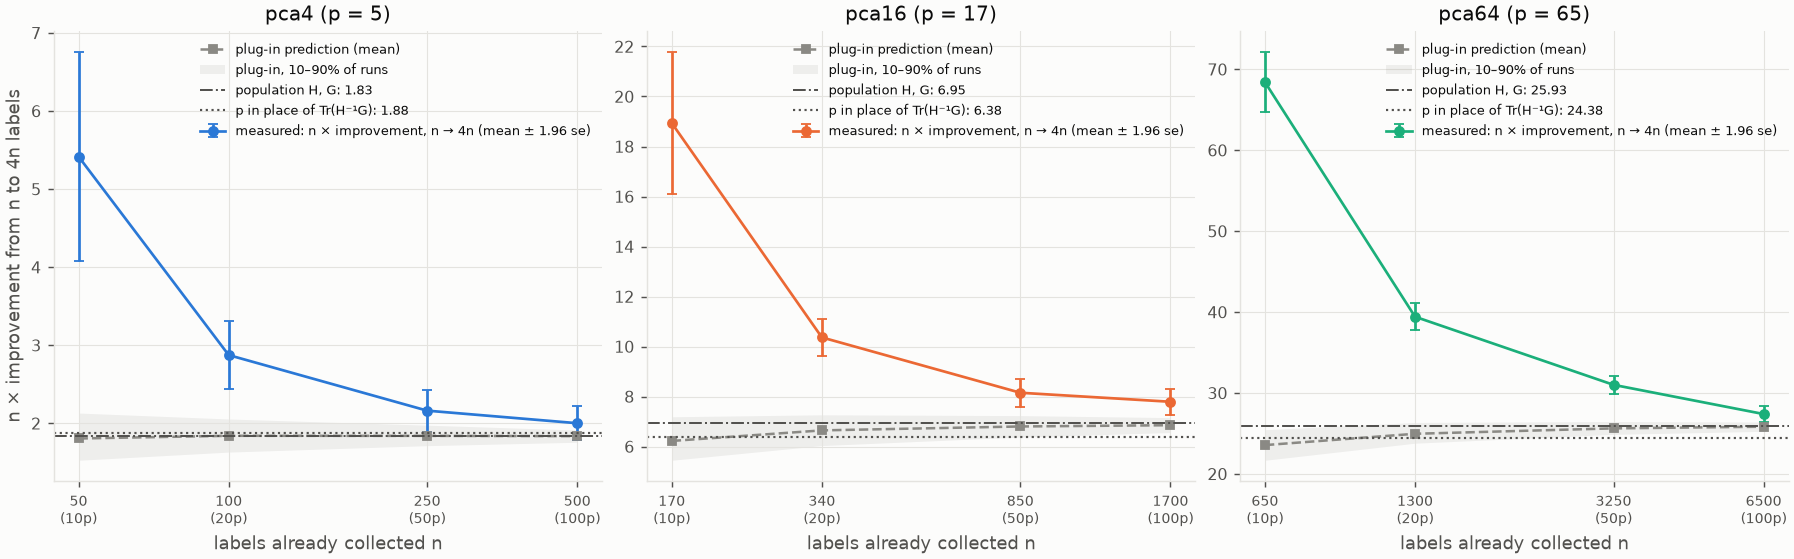
\includegraphics[width=0.8\linewidth]{../figures/e3b_plugin_curve.png}
  \caption{E3b: $n\cdot[L_{\text{test}}(\hat\theta_n)-L_{\text{test}}(\hat\theta_{\EThreeBFactor n})]$
  (mean $\pm1.96$ se), the plug-in prediction (mean and 10--90\% of runs), the same prediction
  with the population $H$, $G$ (dash-dotted) and with $p$ in place of $\Tr(H^{-1}G)$ (dotted).}
  \label{fig:e3b}
\end{figure}
